\begin{figure}[tbp]
\centering
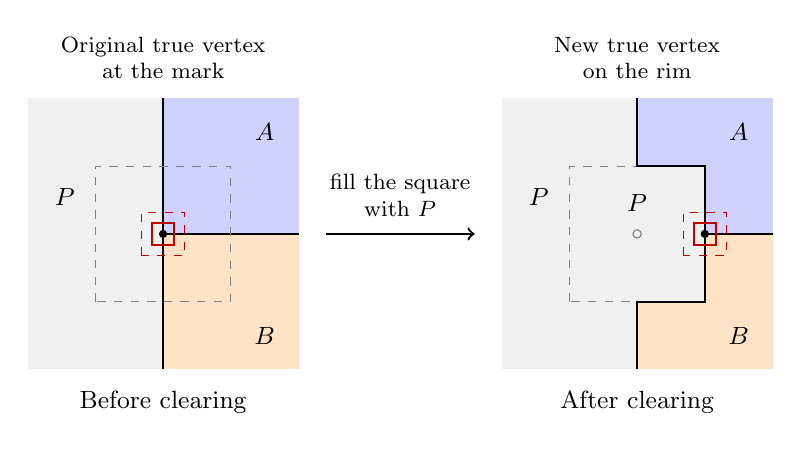
\begin{tikzpicture}[x=0.86cm,y=0.86cm,font=\small]
  \begin{scope}[shift={(-3.5,0)}]
    \fill[gray!12] (-2,-2) rectangle (2,2);
    \fill[blue!18] (0,0) rectangle (2,2);
    \fill[orange!22] (0,-2) rectangle (2,0);
    \draw[thick] (0,-2)--(0,2);
    \draw[thick] (0,0)--(2,0);
    \draw[dashed,gray] (-1,-1) rectangle (1,1);
    \draw[red!75!black,thick] (-0.16,-0.16) rectangle (0.16,0.16);
    \draw[red!75!black,dashed] (-0.32,-0.32) rectangle (0.32,0.32);
    \fill (0,0) circle (1.5pt);
    \node at (-1.45,0.55) {$P$};
    \node at (1.5,1.5) {$A$};
    \node at (1.5,-1.5) {$B$};
    \node[below] at (0,-2.18) {Before clearing};
    \node[above,align=center,font=\footnotesize] at (0,2.15)
      {Original true vertex\\at the mark};
  \end{scope}
  \draw[->,thick] (-1.1,0)--(1.1,0);
  \node[above,align=center,font=\footnotesize] at (0,0.12)
    {fill the square\\with $P$};
  \begin{scope}[shift={(3.5,0)}]
    \fill[gray!12] (-2,-2) rectangle (2,2);
    \fill[blue!18] (0,0) rectangle (2,2);
    \fill[orange!22] (0,-2) rectangle (2,0);
    \fill[gray!12] (-1,-1) rectangle (1,1);
    \draw[dashed,gray] (-1,-1) rectangle (1,1);
    \draw[thick] (0,2)--(0,1)--(1,1)--(1,-1)--(0,-1)--(0,-2);
    \draw[thick] (1,0)--(2,0);
    \draw[red!75!black,thick] (0.84,-0.16) rectangle (1.16,0.16);
    \draw[red!75!black,dashed] (0.68,-0.32) rectangle (1.32,0.32);
    \fill (1,0) circle (1.5pt);
    \draw[gray] (0,0) circle (1.5pt);
    \node at (-1.45,0.55) {$P$};
    \node at (0,0.45) {$P$};
    \node at (1.5,1.5) {$A$};
    \node at (1.5,-1.5) {$B$};
    \node[below] at (0,-2.18) {After clearing};
    \node[above,align=center,font=\footnotesize] at (0,2.15)
      {New true vertex\\on the rim};
  \end{scope}
\end{tikzpicture}
\caption{A point treatment for three distinct labels, shown in units of
$t$.  The dashed gray square is the radius-one treated square; solid
black lines are actual label interfaces.  After filling with $P$, the
only true vertex in this example is the meeting of $P,A,B$ on the right
rim.  The other ray/rim contacts involve only two labels.  Red solid
and dashed squares illustrate the inner and outer holes at the actual
true vertices, enlarged for visibility.  In the protocol their radii are
$h_n$ and $2h_n$, with one uniformly small $\epsilon_0$; the same
construction handles the finitely many ray patterns in the proof.}
\label{fig:geometry-points}
\end{figure}
